\documentclass[12pt]{article}
\usepackage[left=1cm, right=1cm, top=2cm,bottom=1.5cm]{geometry} 

\usepackage[parfill]{parskip}
\usepackage[utf8]{inputenc}
\usepackage[T2A]{fontenc}
\usepackage[russian]{babel}
\usepackage{enumitem}
\usepackage[normalem]{ulem}
\usepackage{amsfonts, amsmath, amsthm, amssymb, mathtools,xcolor}
\usepackage{blkarray}

\usepackage{tabularx}
\usepackage{hhline}

\usepackage{accents}
\usepackage{fancyhdr}
\pagestyle{fancy}
\renewcommand{\headrulewidth}{1.5pt}
\renewcommand{\footrulewidth}{1pt}

\usepackage{graphicx}
\usepackage[figurename=Рис.]{caption}
\usepackage{subcaption}
\usepackage{float}

%%Наименование папки откуда забирать изображения
\graphicspath{ {./images/} }

%%Изменение формата для ввода доказательства
\renewcommand{\proofname}{$\square$  \nopunct}
\renewcommand\qedsymbol{$\blacksquare$}

%%Изменение отступа на таблицах
\addto\captionsrussian{%
	\renewcommand{\proofname}{$\square$ \nopunct}%
}
%% Римские цифры
\newcommand{\RN}[1]{%
	\textup{\uppercase\expandafter{\romannumeral#1}}%
}

%% Для удобства записи
\newcommand{\MR}{\mathbb{R}}
\newcommand{\MC}{\mathbb{C}}
\newcommand{\MQ}{\mathbb{Q}}
\newcommand{\MN}{\mathbb{N}}
\newcommand{\MZ}{\mathbb{Z}}
\newcommand{\MTB}{\mathbb{T}}
\newcommand{\MTI}{\mathbb{I}}
\newcommand{\MI}{\mathrm{I}}
\newcommand{\MCI}{\mathcal{I}}
\newcommand{\MJ}{\mathrm{J}}
\newcommand{\MH}{\mathrm{H}}
\newcommand{\MT}{\mathrm{T}}
\newcommand{\MU}{\mathcal{U}}
\newcommand{\MV}{\mathcal{V}}
\newcommand{\MB}{\mathcal{B}}
\newcommand{\MF}{\mathcal{F}}
\newcommand{\MW}{\mathcal{W}}
\newcommand{\ML}{\mathcal{L}}
\newcommand{\MP}{\mathcal{P}}
\newcommand{\VN}{\varnothing}
\newcommand{\VE}{\varepsilon}
\newcommand{\dx}{\, dx}
\newcommand{\dy}{\, dy}
\newcommand{\dz}{\, dz}
\newcommand{\dd}{\, d}


\theoremstyle{definition}
\newtheorem{defn}{Опр:}
\newtheorem{rem}{Rm:}
\newtheorem{prop}{Утв.}
\newtheorem{exrc}{Упр.}
\newtheorem{problem}{Задача}
\newtheorem{lemma}{Лемма}
\newtheorem{theorem}{Теорема}
\newtheorem{corollary}{Следствие}

\newenvironment{cusdefn}[1]
{\renewcommand\thedefn{#1}\defn}
{\enddefn}

\DeclareRobustCommand{\divby}{%
	\mathrel{\text{\vbox{\baselineskip.65ex\lineskiplimit0pt\hbox{.}\hbox{.}\hbox{.}}}}%
}
%Короткий минус
\DeclareMathSymbol{\SMN}{\mathbin}{AMSa}{"39}
%Длинная шапка
\newcommand{\overbar}[1]{\mkern 1.5mu\overline{\mkern-1.5mu#1\mkern-1.5mu}\mkern 1.5mu}
%Функция знака
\DeclareMathOperator{\sgn}{sgn}

%Функция ранга
\DeclareMathOperator{\rk}{\text{rk}}
\DeclareMathOperator{\diam}{\text{diam}}


%Обозначение константы
\DeclareMathOperator{\const}{\text{const}}

\DeclareMathOperator{\codim}{\text{codim}}

\DeclareMathOperator*{\dsum}{\displaystyle\sum}
\newcommand{\ddsum}[2]{\displaystyle\sum\limits_{#1}^{#2}}

%Интеграл в большом формате
\DeclareMathOperator{\dint}{\displaystyle\int}
\newcommand{\ddint}[2]{\displaystyle\int\limits_{#1}^{#2}}
\newcommand{\ssum}[1]{\displaystyle \sum\limits_{n=1}^{\infty}{#1}_n}

\newcommand{\smallerrel}[1]{\mathrel{\mathpalette\smallerrelaux{#1}}}
\newcommand{\smallerrelaux}[2]{\raisebox{.1ex}{\scalebox{.75}{$#1#2$}}}

\newcommand{\smallin}{\smallerrel{\in}}
\newcommand{\smallnotin}{\smallerrel{\notin}}

\newcommand*{\medcap}{\mathbin{\scalebox{1.25}{\ensuremath{\cap}}}}%
\newcommand*{\medcup}{\mathbin{\scalebox{1.25}{\ensuremath{\cup}}}}%

\makeatletter
\newcommand{\vast}{\bBigg@{3.5}}
\newcommand{\Vast}{\bBigg@{5}}
\makeatother

%Промежуточное значение для sup\inf, поскольку они имеют разную высоту
\newcommand{\newsup}{\mathop{\smash{\mathrm{sup}}}}
\newcommand{\newinf}{\mathop{\mathrm{inf}\vphantom{\mathrm{sup}}}}

%Скалярное произведение
\newcommand{\inner}[2]{\left\langle #1, #2 \right\rangle }
\newcommand{\linsp}[1]{\left\langle #1 \right\rangle }
\newcommand{\linmer}[2]{\left\langle #1 \vert #2\right\rangle }

%Подпись символов снизу
\newcommand{\ubar}[1]{\underaccent{\bar}{#1}}

%% Шапка для букв сверху
\newcommand{\wte}[1]{\widetilde{#1}}
\newcommand{\wht}[1]{\widehat{#1}}

%%Трансформация Фурье
\newcommand{\fourt}[1]{\mathcal{F}\left(#1\right)}
\newcommand{\ifourt}[1]{\mathcal{F}^{-1}\left(#1\right)}

%%Символ вектора
\newcommand{\vecm}[1]{\overrightarrow{#1\,}}

%%Пространстов матриц
\newcommand{\mat}[2]{\operatorname{Mat}_{#1\times #2}}


%%Взятие в скобки, модули и норму
\newcommand{\parfit}[1]{\left( #1 \right)}
\newcommand{\modfit}[1]{\left| #1 \right|}
\newcommand{\sqparfit}[1]{\left\{ #1 \right\}}
\newcommand{\normfit}[1]{\left\| #1 \right\|}

%%Функция для обозначения равномерной сходимости по множеству
\newcommand{\uconv}[1]{\overset{#1}{\rightrightarrows}}
\newcommand{\uconvm}[2]{\overset{#1}{\underset{#2}{\rightrightarrows}}}


%%Функция для обозначения нижнего и верхнего интегралов
\def\upint{\mathchoice%
	{\mkern13mu\overline{\vphantom{\intop}\mkern7mu}\mkern-20mu}%
	{\mkern7mu\overline{\vphantom{\intop}\mkern7mu}\mkern-14mu}%
	{\mkern7mu\overline{\vphantom{\intop}\mkern7mu}\mkern-14mu}%
	{\mkern7mu\overline{\vphantom{\intop}\mkern7mu}\mkern-14mu}%
	\int}
\def\lowint{\mkern3mu\underline{\vphantom{\intop}\mkern7mu}\mkern-10mu\int}

%%След матрицы
\DeclareMathOperator*{\tr}{tr}

\makeatletter
\renewcommand*\env@matrix[1][*\c@MaxMatrixCols c]{%
	\hskip -\arraycolsep
	\let\@ifnextchar\new@ifnextchar
	\array{#1}}
\makeatother


%% Переопределение функции хи, чтобы выглядела более приятно
\makeatletter
\@ifdefinable\@latex@chi{\let\@latex@chi\chi}
\renewcommand*\chi{{\@latex@chi\smash[t]{\mathstrut}}} % want only bottom half of \mathstrut
\makeatletter

\begin{document}
\lhead{Математический анализ - \RN{2}}
\chead{Косухин О.Н.}
\rhead{Семинар - 2}
\section*{Неопределенный интеграл}

Есть два основных метода сведения сложных интегралов к простым: замена переменных и интегрирование по частям.

\subsection*{Замена переменных}
Формула замены переменных происходит из теоремы о дифференцировании сложной функции.

Пусть $F'(x) = f(x)$ на некотором промежутке $\MI$, тогда вместо $x$ можно подставить другую функцию $x = g(t)$, тогда производная сложной функции выражается по формуле:
$$
	\left(F(g(t))\right)' = F'(g(t)){\cdot}g'(t) \Rightarrow \dint f(g(t)){\cdot}g'(t)dt = F(g(t)) +C
$$
Следовательно, если мы умеем считать первообразную от $f(x)$, то мы умеем считать первообразную и от $f(g(t)){\cdot}g'(t)$, следовательно мы сначала считаем интеграл:
$$
	\dint f(x) dx = F(x) + C
$$
И затем подставляем $g(t)$, чтобы получить\textbf{ \uwave{формулу замены переменной}}:
$$
	\dint f(x)dx = \dint f(g(t)){\cdot}g'(t)dt  = F(g(t)) + C
$$
До этого мы узнали частный случай этой формулы замены переменных:
$$
	\dint f(at + b) a{\cdot}dt = F(at + b) + C
$$
\begin{rem}
	Как всегда, надо помнить про промежуток $\inner{a}{b}$ на котором происходит интегрирование. В частности, $g(t)$ должна принимать значения из этого промежутка. Мы об этом вспомним, когда займемся определенными интегралами.
\end{rem}
При замене переменных становится ясно, почему необходимо писать в конце дифференциал по переменной (более подробно об этом станет понятнее, когда будем изучать определенный интеграл):
$$
	\dint f(x) dx = \dint f(g(t)) dg(t) = \dint f(g(t)){\cdot} g'(t)dt
$$

\begin{problem}(\textbf{Д1674})
	$$
		\dint \dfrac{xdx}{\sqrt{1-x^2}}
	$$
\end{problem}
\begin{proof}
	$$
		\dint \dfrac{xdx}{\sqrt{1-x^2}} = \dint \dfrac{t}{\sqrt{1 - t^2}}dt = |g(t) = 1 - t^2, \, g'(t) = -2t| = -\dfrac{1}{2}\dint \dfrac{-2t}{\sqrt{1 - t^2}}dt = 
	$$
	$$
		= -\dfrac{1}{2}\dint \dfrac{1}{\sqrt{g(t)}}{\cdot}g'(t)dt = -\dfrac{1}{2}\dint\dfrac{1}{\sqrt{y}}dy = -\sqrt{y} + C = - \sqrt{1 -x^2} + C
	$$
\end{proof}
\newpage
\begin{problem}(\textbf{Д1680})
	$$
		\dint \dfrac{dx}{(1 + x)\sqrt{x}}, \, \dfrac{dx}{\sqrt{x}} = 2d(\sqrt{x})
	$$
\end{problem}
\begin{proof}
	Пусть $y = \sqrt{x} \Rightarrow dy = \tfrac{1}{2}{\cdot}\tfrac{dx}{\sqrt{x}}$, тогда мы получим:
	$$
		\dint \dfrac{dx}{(1 + x)\sqrt{x}} = \dint \dfrac{2dy}{(1 + y^2 )} = 2 \arctg{y} + C = 2 \arctg{(\sqrt{x})} + C
	$$
\end{proof}

\begin{problem}(\textbf{Д1697})
	$$
		\dint \tg{x} dx
	$$
\end{problem}
\begin{proof}
	$$
		\dint \tg{x} dx = \dint \dfrac{\sin{x}}{\cos{x}}dx = |y = \cos{x}, \, dy = -\sin{x}dx| = -\dint\dfrac{dy}{y} = -\ln|y| + C = - \ln{|\cos{x}|} + C
	$$
\end{proof}
\begin{problem}(\textbf{Д1766})
	$$
		\dint x^2 \sqrt[3]{1 -x} dx
	$$
\end{problem}
\begin{proof}
	Будем пользоваться здесь правилом: если вам что-то не нравится в интеграле, выберете это в качестве новой переменной. Например, здесь $y = \sqrt[3]{1 - x}$, тогда выразим $x$ наоборот:
	$$
		y^3 =  1 - x \Rightarrow x = 1 - y^3, \, dx = -3 y^2 dy
	$$
	Теперь мы можем сделать замену переменной:
	$$
		\dint x^2 \sqrt[3]{1 -x} dx = \dint (1 - y^3)^2 {\cdot} y{\cdot} (-3y^2)dy = -3\dint (1 - y^3)^2 y^3 dy = -3 \dint (y^3 - 2y^6 + y^9)dy =
	$$
	$$
		=  -3{\cdot}\left(\dfrac{y^4}{4} - \dfrac{2y^7}{7} + \dfrac{y^{10}}{10}\right) + C = -3{\cdot}\left(\dfrac{(\sqrt[3]{1 - x})^4}{4} - \dfrac{2(\sqrt[3]{1 - x})^7}{7} + \dfrac{(\sqrt[3]{1 - x})^{10}}{10}\right) + C
	$$
\end{proof}

\begin{problem}(\textbf{Д1776})
	$$
		\dint \dfrac{dx}{\sqrt{1 + e^x}} 
	$$
\end{problem}
\begin{proof}
	Пусть $y = \sqrt{1 + e^x}$, тогда:
	$$
		y^2 = 1 + e^x \Rightarrow e^x = y^2 - 1 \Rightarrow x = \ln{(y^2 - 1)}, \, dx = \dfrac{2y}{y^2 - 1}dy
	$$
	Отметим, что помимо преобразования интегралов тут подразумевается и преобразование некоторых промежутков. Исходный интеграл был определен везде, но при замене мы получаем, что $y > 1$. То есть подразумеваем $y \in (1, + \infty)$ и на этом промежутке замена корректна. Тогда:
	$$
		\dint \dfrac{dx}{\sqrt{1 + e^x}}  = \dint \dfrac{2y dy}{( y^2 - 1){\cdot}y} = 2\dint \dfrac{dy}{y^2 - 1} = 2 {\cdot}\dfrac{1}{2}{\cdot}\ln{\left| \dfrac{y-1}{y+1}\right|} + C =
		\ln{\left| \dfrac{\sqrt{1 + e^x}-1}{\sqrt{1 + e^x}+1}\right|} + C 
	$$ 
\end{proof}
\newpage
\subsection*{Избавление от корней в подстановках}
Попробуем разобраться как избавляться от простейших корней делая подстановки.
\begin{problem}(\textbf{Д1778})
	$$
		\dint \dfrac{dx}{(1 - x^2)^{\frac{3}{2}}} 
	$$
\end{problem}
\begin{proof}
	В данном пример заменой переменной в виде корня, от него не получится избавиться:
	$$
		\sqrt{1 - x^2} =y  \Rightarrow 1 - x^2 = y^2 \Rightarrow 1 - y^2 = x^2 \Rightarrow x = \sqrt{1 - y^2}
	$$
	И когда мы посчитаем дифференциал, то корень может при этом остаться. Поэтому замена в виде корня будет не очень хорошей. В этом случае помогут тригонометрические функции. Мы видим, что $|x| < 1$, следовательно мы можем сделать замену: 
	$$
		x = \sin{t} \Rightarrow 1 - x^2 = 1 - \sin^2{t} = \cos^2{t}
	$$ 
	И следовательно, мы сможем удобно брать корни. Тогда:
	$$
		\sqrt{\cos^2{t}} = |\cos{t}|
	$$
	Поскольку мы можем сами выбирать переменную $t$, то скажем, что мы берем $t \in \left[-\frac{\pi}{2}, \frac{\pi}{2}\right]$, при этом синус пробежит все значения, а косинус будет положительным $\Rightarrow$ можем опустить модуль:
	$$
		\sqrt{\cos^2{t}} = |\cos{t}| = \cos{t}, \, 	x = \sin{t}, \,  dx = \cos{t}dt
	$$
	$$
		\dint \dfrac{dx}{(1 - x^2)^{\frac{3}{2}}} = \dint \dfrac{\cos{t}dt}{\cos^3{t}} = \dint\dfrac{dt}{\cos^2{t}} = \tg{t} + C 
	$$
	Можно подставить в тангенс арксинус и мы получим верный ответ, но попробуем упростить полученный результат:
	$$
		\tg{t} = \dfrac{\sin{t}}{\cos{t}} = \dfrac{x}{\sqrt{1 - x^2}}  \Rightarrow \dint \dfrac{dx}{(1 - x^2)^{\frac{3}{2}}} = \tg{t} + C = \dfrac{x}{\sqrt{1 - x^2}} + C
	$$
\end{proof}

\textbf{Упрощение выражений с $\sqrt{1 - x^2}$}: замена $x = \sin{t}, \, x = \cos{t}$ избавляют нас от корня.

\textbf{Упрощение выражений с $\sqrt{a^2 - x^2}$}: замена $x = a\sin{t}, \, x = a  \cos{t}$ избавляют нас от корня.

Рассмотрим ещё пару замену, позволяющих избавляться от квадратного трехчлена.
\begin{problem}(\textbf{Д1784})
	$$
		\dint \dfrac{dx}{\sqrt{(x - a)(b- x)}}, \quad x - a = (b - a){\cdot}\sin^2{t}
	$$
\end{problem}
\begin{proof}
	$$
		b - x = (b - a) - (x - a) = (b - a) - (b - a){\cdot}\sin^2{t} = (b-a){\cdot}\cos^2{t}
	$$
	Без потери общности будем считать, что $a < b$. Поскольку наш трехчлен имеет вид: $(x - a)(b - x)$, то он положителен только на интервале $(a,b) \Rightarrow $ подразумевается, что мы работаем на этом интервале. 
	\begin{figure}[H]
		\centering
		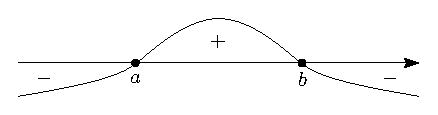
\includegraphics[width=0.45\textwidth]{MA2S2_1.eps}
		\caption{Значения квадратного трехчлена $(x-a)(b-x)$ на $\MR$.}
		\label{2_1}
	\end{figure}
	Выберем значения $t \in \left(0,\frac{\pi}{2}\right)$, тогда: 
	$$
		t \in \left(0,\frac{\pi}{2}\right) \Rightarrow \sin^2{t} \in (0,1) \Rightarrow (b-a)\sin^2{t} \in (0, b-a) \Rightarrow x = a + (b-a)\sin^2{t} \in (a,b)
	$$
	$$
		\dint \dfrac{dx}{\sqrt{(x - a)(b- x)}} = \dint \dfrac{dx}{ \sqrt{(b-a)^2\sin^2{t}\cos^2{t}}} = 
	$$
	$$	
		=\dint \dfrac{(b -a)2\cos{t}\sin{t}dt}{(b-a)\sin{t}\cos{t}} = 2t + C = 2\arcsin{\sqrt{\dfrac{x-a}{b-a}}} + C
	$$
\end{proof}
Также, иногда от корня помогают гиперболические замены переменных. Вспомним, что:
$$
	\sh{t} = \dfrac{e^t - e^{-t}}{2}, \, \ch{t} = \dfrac{e^t + e^{-t}}{2}, \, \ch^2{t} - \sh^2{t} = 1
$$
\begin{problem}(\textbf{Д1786})
	$$
		\dint \sqrt{a^2 + x^2} dx
	$$
\end{problem}
\begin{proof}
	Сделаем замену $x = a \sh{t} \Rightarrow  dx = a\ch{t}dt $, тогда: 
	$$
		a^2 + x^2 = a^2 + a^2\sh^2{t} = a^2\ch^2{t} \Rightarrow \sqrt{a^2 + x^2} = \sqrt{a^2\ch^2{t}} = a\ch{t}
	$$
	В данном случае, даже не важно, какие $t$ мы берем, поскольку $\ch{t} > 0$.
	$$
		 \dint \sqrt{a^2 + x^2} dx = \dint a\ch{t}{\cdot} a \ch{t}dt = a^2\dint \ch^2{t}dt = \dfrac{a^2}{4}\dint (e^t + e^{-t})^2 dt
	$$
	И дальше взять интеграл по стандартным правилам. Но можно и воспользоваться соотношенями, которые есть для гиперболических функций:
	$$
		\ch{2t} = \dfrac{e^{2t} + e^{-2t}}{2} = 2 {\cdot}\dfrac{e^{2t} + e^{-2t} + 2}{4} - 1 = 2\dfrac{(e^t + e^{-t})^2}{4} - 1 = 2\ch^2{t} - 1 \Rightarrow
	$$
	$$
		\Rightarrow a^2\dint \ch^2{t}dt = \dfrac{a^2}{2} \dint (\ch{(2t)} + 1)dt = \dfrac{a^2t}{2} + \dfrac{a^2}{4}\sh{(2t)} + C
	$$
	Также мы знаем, что $\sh{(2t)} = 2\sh{t}\ch{t}$: 
	$$
		\sh{(2t)} = \dfrac{e^{2t} - e^{-2t}}{2} = \dfrac{(e^{t} - e^{-t}){\cdot}(e^t + e^{-t})}{2} = 2{\cdot}\dfrac{e^{t} - e^{-t}}{2}{\cdot}\dfrac{e^{t} + e^{-t}}{2} = 2\sh{t}{\cdot}\ch{t}
	$$
	Тогда, наше выражение с $\sh{(2t)}$ примет вид:
	$$
		x = a\sh{t} \Rightarrow \sh{t} = \dfrac{x}{a}, \, \ch{t} = \dfrac{1}{a}{\cdot}\sqrt{a^2 + x^2} \Rightarrow \sh{(2t)} = 2\sh{t}\ch{t} = 2 {\cdot}\dfrac{x}{a}{\cdot}\dfrac{1}{a}{\cdot}\sqrt{a^2 + x^2}
	$$
	Тогда получим ответ после подстановки ареасинуса $t= \ln{\left(\tfrac{x}{a} + \sqrt{\left(\tfrac{x}{a}\right)^2 + 1}\right)}$:
	$$
		\dint \sqrt{a^2 + x^2} dx =  \dfrac{a^2}{2}\left(\ln{\left(\dfrac{x}{a} + \sqrt{\left(\dfrac{x}{a}\right)^2 + 1}\right)} +  \dfrac{x}{a^2}{\cdot}\sqrt{a^2 + x^2}\right) + C
	$$
\end{proof}

\textbf{Упрощение выражений с $\sqrt{a^2 + x^2}$}: замена $x = a\sh{t}$ избавляют нас от корня.

\textbf{Упрощение выражений с $\sqrt{x^2 - a^2}$}: замена $x = a\ch{t}$ избавляют нас от корня.

\subsection*{Интегрирование по частям}
Данный метод основывается на правиле производной произведения:
$$
	(u(t){\cdot}v(t))' = u'(t){\cdot}v(t) + u(t){\cdot}v'(t) \Rightarrow \dint u'(t){\cdot}v(t) + u(t){\cdot}v'(t) dt = u(t){\cdot}v(t) + C
$$
По линейности, при существовании интеграла от слагаемого (интеграл от другого существует, потому что интеграл от суммы существует) мы получим:
$$
	\dint u'(t){\cdot}v(t) dt = u(t){\cdot}v(t) - \dint u(t){\cdot}v'(t) dt
$$
Это \textbf{\uwave{формула интегрирования по частям}}. 
\begin{rem}
	Возникает вопрос, почему мы не пишем плюс $C$? Мы его не пишем, поскольку в формуле написано равенство двух множеств.
\end{rem}
 \begin{problem}(\textbf{Д1791})
 	$$
 		\dint \ln{x} dx
 	$$
 \end{problem}
\begin{proof}
	$$
		\dint \ln{x} dx =  \dint 1{\cdot}\ln{x} dx, \, 1 = u'(x) \Rightarrow u(x) = x, \, \ln{x} = v(x) \Rightarrow 
	$$
	$$
		\Rightarrow \dint \ln{x} dx = x{\cdot}\ln{x} - \dint x{\cdot}\dfrac{1}{x}dx = x\ln{x} - x + C
	$$
\end{proof}
\textbf{Когда надо применять интегрирование по частям}: очень часто это нужно делать, когда мы видим обратную функцию, например:
$$
	\ln{x}, \, \log_a{x}, \, \arccos{x}, \, \arcsin{x}, \, \arctg{x}, \, \arcctg{x}, \, \sh^{-1}{x}, \, \ch^{-1}{x}, \, \th^{-1}{x}, \, \cth^{-1}{x}
$$
Также метод применяется, когда мы видим два разнородных множителя, например:
$$
	x{\cdot}e^x, \, x{\cdot}\sin{x}, \, x^2{\cdot}\cos{x}, \, e^{x}{\cdot}\sin{x}
$$
\newpage
\begin{problem}(\textbf{Д1796})
	$$
		\dint x^2 e^{-2x}dx
	$$
\end{problem}
\begin{proof}
	Мы видим, что у нас произведение двух разноплановых множителей: есть степенная функция, есть показательная функция $\Rightarrow$ намёк на то, что нужно использовать интегрирование по частям. Обозначим функции следующим образом:
	$$
		v(x) = x^2, \, u'(x) = e^{-2x} \Rightarrow u(x) = \dfrac{-e^{-2x}}{2}
	$$
	Тогда по формуле интегрирования по частям:
	$$
		\dint x^2 e^{-2x}dx = -\dfrac{x^2}{2}e^{-2x} + \dfrac{1}{2}\dint e^{-2x}{\cdot}2x dx = -\dfrac{x^2}{2}e^{-2x} + \dint e^{-2x}x dx
	$$
	Воспользуемся формулой ещё раз:
	$$
		-\dfrac{x^2}{2}e^{-2x} + \dint e^{-2x}x dx = -\dfrac{x^2}{2}e^{-2x} + \left(-\dfrac{x}{2}e^{-2x} + \dfrac{1}{2}\dint e^{-2x}dx\right) = -e^{-2x}{\cdot}\left(\dfrac{x^2}{2} + \dfrac{x}{2} + \dfrac{1}{4}\right) + C
	$$
\end{proof}

\begin{problem}(\textbf{Д1828})
	$$
		\dint e^{ax} \cos{bx}dx
	$$
\end{problem}
\begin{proof}
	Потребуем, чтобы $a, b \neq 0$, иначе это будет  более простой интеграл и его можно просто посчитать. Видим, что здесь разнородные функции. Обозначим функции следующим образом:
	$$
		v(x) = \cos{bx}, \, u'(x) = e^{ax} \Rightarrow u(x) = \dfrac{1}{a}e^{ax}
	$$
	Тогда по формуле интегрирования по частям:
	$$
		\dint e^{ax} \cos{bx}dx = \dfrac{1}{a}e^{ax}\cos{bx} + \dfrac{b}{a}\dint e^{ax} \sin{bx}dx
	$$
	Воспользуемся формулой ещё раз, снова обозначив $u'(x) = e^{ax}, \, v(x) = \sin{bx}$, тогда:
	$$
		\dfrac{1}{a}{\cdot}e^{ax}{\cdot}\cos{bx} + \dfrac{b}{a}{\cdot}\dint e^{ax}{\cdot} \sin{bx}dx = \dfrac{1}{a}{\cdot}e^{ax}{\cdot}\cos{bx} + \dfrac{b}{a}{\cdot}\left(\dfrac{1}{a}{\cdot}e^{ax}{\cdot}\sin{bx} - \dfrac{b}{a}{\cdot}\dint e^{ax}{\cdot}\cos{bx}dx\right)
	$$
	Обозначим исходный интеграл через $\MI$, тогда мы получим:
	$$
		\MI = \dfrac{1}{a}{\cdot}e^{ax}{\cdot}\cos{bx} + \dfrac{b}{a^2}{\cdot}e^{ax}{\cdot}\sin{bx} - \dfrac{b^2}{a^2}{\cdot}\MI \Rightarrow \MI \left(\dfrac{a^2 + b^2}{a^2}\right) = \dfrac{e^{ax}}{a}{\cdot}\left(\cos{bx} + \dfrac{b}{a} \sin{bx}\right) + C
	$$
	Тогда мы получим:
	$$
		\MI = \dint e^{ax} \cos{bx}dx = e^{ax}{\cdot}\left(\dfrac{a}{a^2 + b^2}\cos{bx} + \dfrac{b}{a^2 + b^2}\sin{bx}\right) + C
	$$
\end{proof}
\begin{rem}
	В задаче выше надо никогда не забывать, что равенства без $C$ это равенства по множествам. 
\end{rem}

\textbf{ДЗ}: $1690, \, 1695, \, 1703$ (перейти к половинному углу: $\sin{x} = 2\sin{\frac{x}{2}}\cos{\frac{x}{2}}$, замена $t= \tg{\frac{x}{2}}$). 

\textbf{ДЗ}: подстановки: $1777, \, 1780, \, 1785, \, 1790, \, 1829$.

\end{document}